\documentclass[tikz,border=5mm]{standalone}
\usepackage{tikz}
\usetikzlibrary{positioning,arrows.meta}
\usepackage{xcolor}
\usepackage{amssymb}

% Define colors
\definecolor{nodefcolor}{RGB}{220,53,69}
\definecolor{patterncolor}{RGB}{255,193,7}
\definecolor{policycolor}{RGB}{0,123,255}
\definecolor{provsafecolor}{RGB}{40,167,69}
\definecolor{gridcolor}{RGB}{200,200,200}
\definecolor{secondary}{RGB}{108,117,125}

\begin{document}
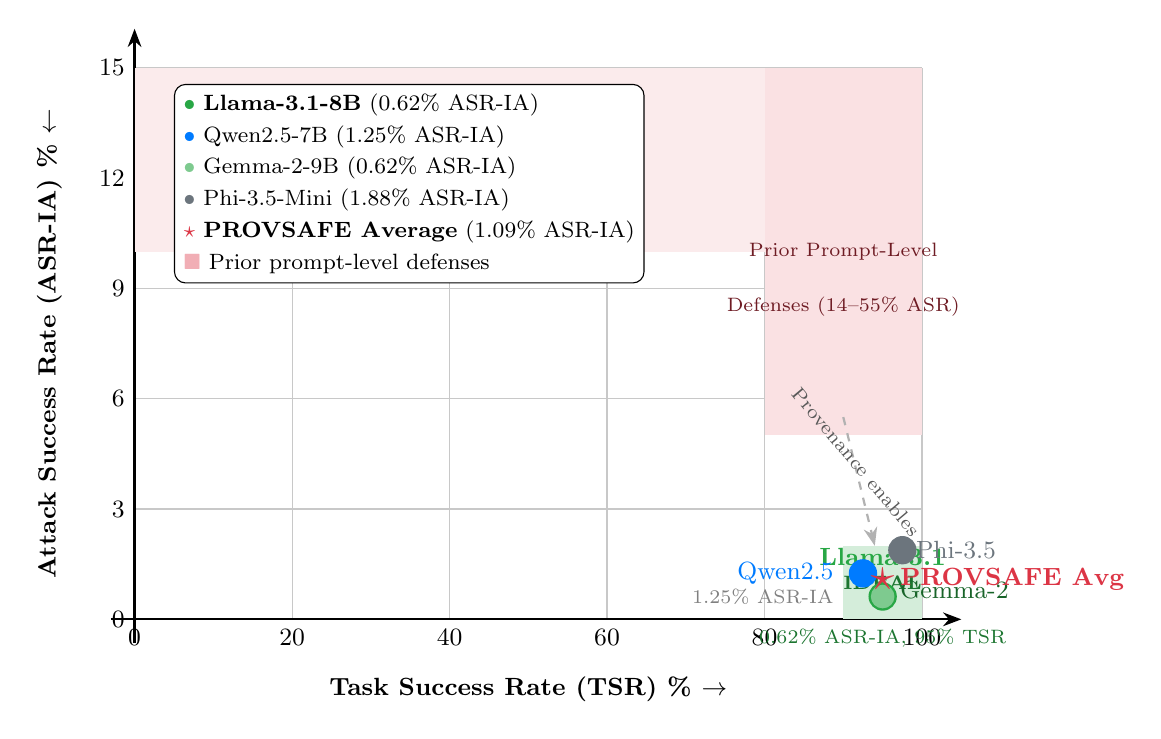
\begin{tikzpicture}[
    >=Stealth
]

% Grid dimensions: 10cm x 7cm
% X axis: TSR 0-100%, scaled to 10cm
% Y axis: ASR 0-15%, scaled to 7cm (0.467cm per %)

\def\xscale{0.1}  % 10cm / 100%
\def\yscale{0.467} % 7cm / 15%

% Draw grid
\foreach \x in {0,20,40,60,80,100} {
    \draw[gridcolor] (\x*\xscale, 0) -- (\x*\xscale, 15*\yscale);
    \node[below, font=\small] at (\x*\xscale, 0) {\x};
}
\foreach \y in {0,3,6,9,12,15} {
    \draw[gridcolor] (0, \y*\yscale) -- (100*\xscale, \y*\yscale);
    \node[left, font=\small] at (0, \y*\yscale) {\y};
}

% Axes
\draw[->, thick] (-0.3,0) -- (10.5,0);
\draw[->, thick] (0,-0.3) -- (0,7.5);

% Axis labels
\node[below, font=\small\bfseries] at (5, -0.6) {Task Success Rate (TSR) \% $\rightarrow$};
\node[left, font=\small\bfseries, rotate=90, anchor=south] at (-0.8, 3.5) {Attack Success Rate (ASR-IA) \% $\leftarrow$};

% Ideal region
\fill[provsafecolor!20] (90*\xscale, 0) rectangle (100*\xscale, 2*\yscale);
\node[font=\scriptsize\bfseries, provsafecolor!70!black] at (95*\xscale, 1*\yscale) {IDEAL};

% Dangerous region
\fill[nodefcolor!10] (0, 10*\yscale) rectangle (100*\xscale, 15*\yscale);
\node[font=\scriptsize, nodefcolor!50!black] at (50*\xscale, 13*\yscale) {High Risk Zone};

% Data points
% Llama-3.1-8B: TSR=95.0, ASR=0.62
\fill[provsafecolor] (95.0*\xscale, 0.62*\yscale) circle (0.18);
\node[anchor=south, font=\small\bfseries, provsafecolor] at (95.0*\xscale, 1.2*\yscale) {Llama-3.1};
\node[anchor=north, font=\scriptsize, provsafecolor!70!black] at (95.0*\xscale, 0.0*\yscale) {0.62\% ASR-IA, 95\% TSR};

% Qwen2.5-7B: TSR=92.5, ASR=1.25
\fill[policycolor] (92.5*\xscale, 1.25*\yscale) circle (0.18);
\node[anchor=east, font=\small, policycolor] at (90*\xscale, 1.25*\yscale) {Qwen2.5};
\node[anchor=east, font=\scriptsize, gray] at (90*\xscale, 0.6*\yscale) {1.25\% ASR-IA};

% Gemma-2-9B: TSR=95.0, ASR=0.62
\fill[provsafecolor!60] (95.0*\xscale, 0.62*\yscale) circle (0.15);
\node[anchor=south west, font=\small, provsafecolor!60!black] at (96*\xscale, 0.3*\yscale) {Gemma-2};

% Phi-3.5-Mini: TSR=97.5, ASR=1.88
\fill[secondary] (97.5*\xscale, 1.88*\yscale) circle (0.18);
\node[anchor=west, font=\small, secondary] at (98*\xscale, 1.88*\yscale) {Phi-3.5};

% PROVSAFE Average: TSR=95.00, ASR=1.09
\node[nodefcolor, font=\LARGE] at (95.00*\xscale, 1.09*\yscale) {$\star$};
\node[anchor=west, font=\small\bfseries, nodefcolor] at (96*\xscale, 1.09*\yscale) {PROVSAFE Avg};

% Prior work region (approximate)
\fill[nodefcolor!15] (80*\xscale, 5*\yscale) rectangle (100*\xscale, 15*\yscale);
\node[font=\scriptsize, nodefcolor!50!black] at (90*\xscale, 10*\yscale) {Prior Prompt-Level};
\node[font=\scriptsize, nodefcolor!50!black] at (90*\xscale, 8.5*\yscale) {Defenses (14--55\% ASR)};

% Arrow from prior work to PROVSAFE
\draw[->, thick, gray!60, dashed] (90*\xscale, 5.5*\yscale) -- (94*\xscale, 2.0*\yscale);
\node[above, font=\scriptsize, gray!70!black, rotate=-50] at (90*\xscale, 4*\yscale) {Provenance enables};

% Legend box
\node[draw, rounded corners, fill=white, font=\footnotesize, align=left, anchor=north west] at (0.5, 6.8) {
    \textcolor{provsafecolor}{$\bullet$} \textbf{Llama-3.1-8B} (0.62\% ASR-IA)\\[2pt]
    \textcolor{policycolor}{$\bullet$} Qwen2.5-7B (1.25\% ASR-IA)\\[2pt]
    \textcolor{provsafecolor!60}{$\bullet$} Gemma-2-9B (0.62\% ASR-IA)\\[2pt]
    \textcolor{secondary}{$\bullet$} Phi-3.5-Mini (1.88\% ASR-IA)\\[2pt]
    \textcolor{nodefcolor}{$\star$} \textbf{PROVSAFE Average} (1.09\% ASR-IA)\\[2pt]
    \textcolor{nodefcolor!40}{$\blacksquare$} Prior prompt-level defenses
};

\end{tikzpicture}
\end{document}
